\section{Estimating Speciation \& Extinction Rates Through Time}

\subsection{Outline}

This tutorial describes how to specify an episodic branching-process model in \RevBayes; a birth-death process where diversification rates vary episodically through time modeled as piecewise-constant rates \citep{Stadler2011,Hoehna2015a}.
The probabilistic graphical model is given once at the beginning of this tutorial.
Your goal is to estimate speciation and extinction rates through-time using Markov chain Monte Carlo (MCMC).


\subsection{Requirements}
We assume that you have read and hopefully completed the following tutorials:
\begin{itemize}
\item \href{https://github.com/revbayes/revbayes_tutorial/raw/master/tutorial_TeX/RB_Getting_Started/RB_Getting_Started.pdf}{Getting started}
\item \href{https://github.com/revbayes/revbayes_tutorial/raw/master/tutorial_TeX/RB_Basics_Tutorial/RB_Basics_Tutorial.pdf}{\Rev basics}
\item \href{https://github.com/revbayes/revbayes_tutorial/raw/master/tutorial_TeX/RB_DiversificationRate_Tutorial/RB_DiversificationRate_Tutorial.pdf}{Basic Diversification Rate Estimation}
\end{itemize}
Note that the \href{https://github.com/revbayes/revbayes_tutorial/raw/master/tutorial_TeX/RB_Basics_Tutorial/RB_Basics_Tutorial.pdf}{\Rev basics tutorial} introduces the basic syntax of \Rev but does not cover any phylogenetic models.
You may skip the \href{https://github.com/revbayes/revbayes_tutorial/raw/master/tutorial_TeX/RB_Basics_Tutorial/RB_Basics_Tutorial.pdf}{\Rev basics tutorial} if you have some familiarity with \R.
We tried to keep this tutorial very basic and introduce all the language concepts and theory on the way.
You may only need the \href{https://github.com/revbayes/revbayes_tutorial/raw/master/tutorial_TeX/RB_Basics_Tutorial/RB_Basics_Tutorial.pdf}{\Rev basics tutorial} for a more in-depth discussion of concepts in \Rev.


%%%%%%%%
%%   Data   %%
%%%%%%%%
\section{Data and files}

We provide the data file(s) which we will use in this tutorial.
You may want to use your own data instead.
In the \cl{data} folder, you will find the following files
\begin{itemize}
\item \cl{primates\_tree.nex}: Dated primates phylogeny including 233 out of 367 species from \cite{MagnusonFord2012}.
\end{itemize}


\impmark{Open the tree \cl{data/primates\_tree.nex} in \FigTree.}


\bigskip
\section{Episodic Birth-Death Model}

The basic idea behind the model is that speciation and extinction rates are constant within time intervals but can be different between time intervals.
Thus, we will divide time into equally sized intervals, with the only exception that the first 20\% of the time does not have any rate changes.
Our only reason to do so is because there are too few lineages in the reconstructed tree at that time to obtain reliable parameter estimates.
An overview of the underlying theory of the specific model and implementation is given in \cite{Hoehna2015a}.
\begin{figure}[h!]
\centering
\fbox{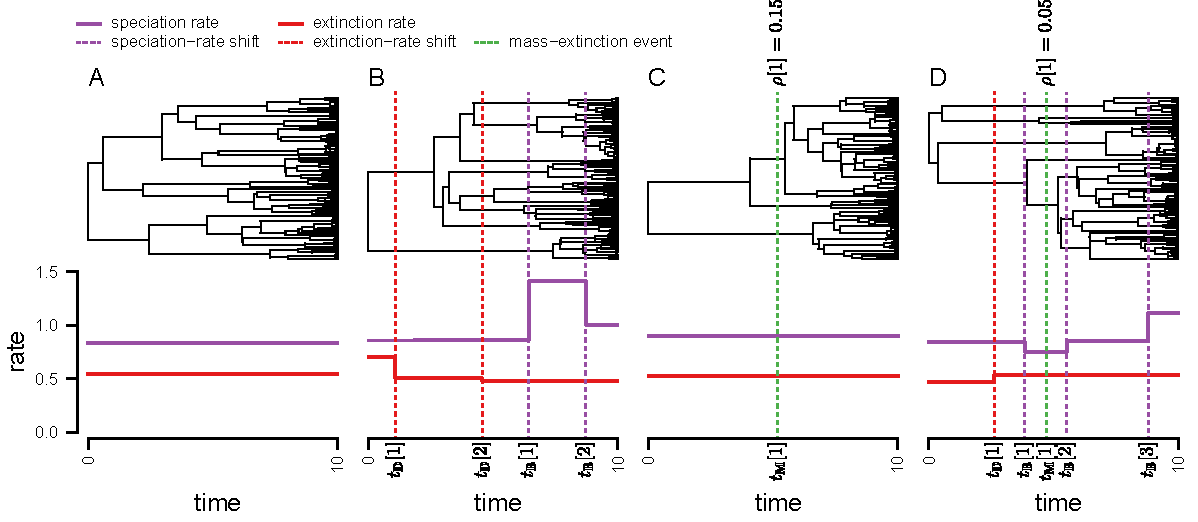
\includegraphics[width=\textwidth]{\ResourcePath figures/EBD_scenarios.pdf}}
\caption{\small Two scenarios of birth-death models. On the left we show constant diversification. On the right we show an example of an episodic birth-death process where rates are constant in each time interval (epoch). The top panel of this figure shows an example realization under the given rates.}
\label{fig:EBD}
\end{figure}
Figure~\ref{fig:EBD} shows an example of a constant rate birth-death process and an episodic birth-death process.

We assume that the log-transformed rates are drawn from a normal distribution.
Furthermore, we will assume that rates are autocorrelated, that is, rates in the current time interval will be centered around the rates in the previous time interval.
Thus, we model (log-transformed) diversification rates by a Brownian motion.
The assumption of autocorrelated rates does not only makes sense biologically but also improves our ability to estimate parameters.
\begin{figure}[h!]
\centering
\fbox{\includegraphics[width=\textwidth]{\ResourcePath figures/Graphical_Model_EBD.pdf}}
\caption{\small A graphical model with the outline of the \Rev code. On the left we see the graphical model describing the correlated (Brownian motion) model for rate-variation through time. On the right we show the corresponding \Rev commands to instantiate this model. This figure gives a complete overview of the model that we use here in this analysis.}
\label{fig:EBD_GM}
\end{figure}
We show a graphical model of the episodic birth-death process with autocorrelated rates in Figure~\ref{fig:EBD_GM}.
This graphical model shows you which variables are included in the model, and the dependency between the variables.
Thus, it makes the structure and assumption of the model clear and visible instead of a black-box \citep{Hoehna2014b}.
For example, you see how the speciation and extinction rates in each time interval depend on the rates of the previous interval, and that we use a hyperprior for the standard deviation of rates between time intervals.


\subsection{Read the tree}

Begin by reading in the ``observed'' tree.

{\tt \begin{snugshade*}
\begin{lstlisting}
T <- readTrees("data/primates_tree.nex")[1]
\end{lstlisting}
\end{snugshade*}}

From this tree, we get some helpful variables, such as the taxon information which we need to instantiate the birth-death process.
{\tt \begin{snugshade*}
\begin{lstlisting}
taxa <- T.taxa()
\end{lstlisting}
\end{snugshade*}}

Additionally, we initialize an iterator variable for our vector of moves and monitors.
{\tt \begin{snugshade*}
\begin{lstlisting}
mvi = 0
mni = 0
\end{lstlisting}
\end{snugshade*}}

Finally, we create a helper variable that specifies the number of intervals.
{\tt \begin{snugshade*}
\begin{lstlisting}
NUM_INTERVALS = 10
\end{lstlisting}
\end{snugshade*}}
Using this variable we can easily change our script to break-up time into many (\EG~\cl{NUM\_INTERVALS = 100}) or few (\EG~\cl{NUM\_INTERVALS = 4}) intervals.



\subsection{Specifying the model}

\subsubsection{Priors on amount of rate variation}
We start by specifying prior distributions on the rates.
Each interval-specific speciation- and extinction-rate will be drawn from a normal distribution.
Thus, we need a parameter for the standard deviation of those normal distributions.
We use an exponential hyperprior with rate 1.0 to estimate the standard deviation, but assume that all speciation rates and all extinction rates share the same standard deviation.
The motivation for an exponential hyperprior is that it has the highest probability density at 0 which would make the variance of rates between consecutive time intervals 0 and thus represent a constant-rate process.
The data will tell us if there should be much variation in rates through time.
(You may want to experiment with this hyperprior if you are interested.)
{\tt \begin{snugshade*}
\begin{lstlisting}
speciation_sd ~ dnExponential(1.0)
extinction_sd ~ dnExponential(1.0)
\end{lstlisting}
\end{snugshade*}}
We apply a simple scaling move on each prior parameter.
{\tt \begin{snugshade*}
\begin{lstlisting}
moves[++mvi] = mvScale(speciation_sd,weight=5.0)
moves[++mvi] = mvScale(extinction_sd,weight=5.0)
\end{lstlisting}
\end{snugshade*}}



\subsubsection{Specifying episodic rates}
As we mentioned before, we will apply normal distributions as priors for each log-transformed rate.
We begin with the rate at the present which is our initial rate parameter.
The rates at the present will be specified slightly differently because they are not correlated to any previous rates.
This is because we are actually modeling rate-changes backwards in time and there is no previous rate for the rate at the present.
Modeling rates backwards in time makes it easier for us if we had some prior information about some event affected diversification sometime before the present, \EG 25 million years ago.

We use a uniform distribution between -10 and 10 because of our lack of prior knowledge on the diversification rate.
This actually means that we allow speciation and extinction rates between $e^{-10}$ and $e^10$, so we should clearly cover the true values.
(Note that for diversification rate estimates, $e^{-10}$ is virtually 0 since the rate is so slow).
{\tt \begin{snugshade*}
\begin{lstlisting}
log_speciation[1] ~ dnUniform(-10.0,10.0)
log_speciation[1] ~ dnUniform(-10.0,10.0)
\end{lstlisting}
\end{snugshade*}}
Notice that we store the diversification rate variables in vectors.
Storing the rate parameters in vectors will be useful and important later when we pass the rates into the birth-death process.

We apply simple sliding window moves for the rates.
Normally we would use scaling moves but in this case we work on the log-transformed parameters and thus sliding moves perform better.
(If you are keen you can test the differences.)
{\tt \begin{snugshade*}
\begin{lstlisting}
moves[++mvi] = mvSlide(log_speciation[1], weight=2)
moves[++mvi] = mvSlide(log_extinction[1], weight=2)
\end{lstlisting}
\end{snugshade*}}
Now we transform the diversification rate parameters into actual rates using an exponential parameter transformation.
{\tt \begin{snugshade*}
\begin{lstlisting}
speciation[1] := exp( log_speciation[1] )
extinction[1] := exp( log_extinction[1] )
\end{lstlisting}
\end{snugshade*}}

Next, we specify the speciation and extinction rates for each time interval (\IE epoch).
This can be done efficiently using a \cl{for}-loop.
We will use a specific index variable so that we can more easily refer to the rate at the previous interval.
Remember that we want to model the rates as a Brownian motion, which we achieve by specifying a normal distribution as the prior distribution on the rates centered around the previous rate (\IE the mean of the normal distribution is equal to the previous rate).
{\tt \begin{snugshade*}
\begin{lstlisting}
for (i in 1:NUM_INTERVALS) {
    index = i+1

    log_speciation[index] ~ dnNormal( mean=log_speciation[i], sd=speciation_sd )
    log_extinction[index] ~ dnNormal( mean=log_extinction[i], sd=extinction_sd )

    moves[++mvi] = mvSlide(log_speciation[index], weight=2)
    moves[++mvi] = mvSlide(log_extinction[index], weight=2)

    speciation[index] := exp( log_speciation[index] )
    extinction[index] := exp( log_extinction[index] )

}
\end{lstlisting}
\end{snugshade*}}
Finally, we apply moves that slide all values in the rate vectors, \IE all speciation or extinction rates.
We will use an \cl{mvVectorSlide} move.
{\tt \begin{snugshade*}
\begin{lstlisting}
moves[++mvi] = mvVectorSlide(log_speciation, weight=10)
moves[++mvi] = mvVectorSlide(log_extinction, weight=10)
\end{lstlisting}
\end{snugshade*}}

Additionally, we apply a \cl{mvShrinkExpand} move which changes the spread of several variables around their mean.
{\tt \begin{snugshade*}
\begin{lstlisting}
moves[++mvi] = mvShrinkExpand( log_speciation, sd=speciation_sd, weight=10 )
moves[++mvi] = mvShrinkExpand( log_extinction, sd=extinction_sd, weight=10 )
\end{lstlisting}
\end{snugshade*}}
Both moves considerably improve the efficiency of our MCMC analysis.

\subsubsection{Setting up the time intervals}
In \RevBayes you actually have the possibility to specify unequal time intervals or even different intervals for the speciation and extinction rate.
This is achieved by providing a vector of times when each interval ends.
Here we simply break-up the most recent 80\% of time since the root in equal-length intervals.
{\tt \begin{snugshade*}
\begin{lstlisting}
interval_times <- T.rootAge() * (1:NUM_INTERVALS) / (NUM_INTERVALS) * 0.8
\end{lstlisting}
\end{snugshade*}}
This vector of times will be used for both the speciation and extinction rates.
Also, remember that the times of the intervals represent ages going backwards in time.

\subsubsection{Incomplete Taxon Sampling}

We know that we have sampled 233 out of 367 living primate species.
To account for this we can set the sampling parameter as a constant node with a value of 233/367.
For simplicity, and since almost all species have been sampled, we assume \emph{uniform} taxon sampling \citep{Hoehna2011,Hoehna2014a},
{\tt \begin{snugshade*}
\begin{lstlisting}
rho <- T.ntips()/367
\end{lstlisting}
\end{snugshade*}}


\subsubsection{Root age}

The birth-death process requires a parameter for the root age.
In this exercise we use a fixed tree and thus we know the age of the tree.
Hence, we can get the value for the root from the \citet{MagnusonFord2012} tree.
{\tt \begin{snugshade*}
\begin{lstlisting}
root_time <- T.rootAge()
\end{lstlisting}
\end{snugshade*}}

\subsubsection{The time tree}

Now we have all of the parameters we need to specify the full episodic birth-death model.
We initialize the stochastic node representing the time tree.
{\tt \begin{snugshade*}
\begin{lstlisting}
timetree ~ dnEpisodicBirthDeath(rootAge=T.rootAge(), lambdaRates=speciation, lambdaTimes=interval_times, muRates=extinction, muTimes=interval_times, rho=rho, samplingStrategy="uniform", condition="survival", taxa=taxa)
\end{lstlisting}
\end{snugshade*}}
You may notice that we explicitly specify that we want to condition on survival.
It is possible to change this condition to the \emph{time of the process} or \emph{the number of sampled taxa} too.

Then we attach data to the \cl{timetree} variable.
{\tt \begin{snugshade*}
\begin{lstlisting}
timetree.clamp(T)
\end{lstlisting}
\end{snugshade*}}

Finally, we create a workspace object of our whole model using the \cl{model()} function.
{\tt \begin{snugshade*}
\begin{lstlisting}
mymodel = model(speciation)
\end{lstlisting}
\end{snugshade*}}

The \cl{model()} function traversed all of the connections and found all of the nodes we specified.


\subsection{Running an MCMC analysis}

\subsubsection{Specifying Monitors}

For our MCMC analysis, we need to set up a vector of \textit{monitors} to record the states of our Markov chain.
First, we will initialize the model monitor using the \cl{mnModel} function. This creates a new monitor variable that will output the states for all model parameters when passed into a MCMC function.
{\tt \begin{snugshade*}
\begin{lstlisting}
monitors[++mni] = mnModel(filename="output/primates_EBD.log",printgen=10, separator = TAB)
\end{lstlisting}
\end{snugshade*}}

Additionally, we create four separate file monitors, one for each vector of speciation and extinction rates and for each speciation and extinction rate epoch (\IE the times when the interval ends).
We want to have the speciation and extinction rates stored separately so that we can plot them nicely afterwards.
{\tt \begin{snugshade*}
\begin{lstlisting}
monitors[++mni] = mnFile(filename="output/primates_EBD_speciation_rates.log",printgen=10, separator = TAB, speciation)
monitors[++mni] = mnFile(filename="output/primates_EBD_speciation_times.log",printgen=10, separator = TAB, interval_times)
monitors[++mni] = mnFile(filename="output/primates_EBD_extinction_rates.log",printgen=10, separator = TAB, extinction)
monitors[++mni] = mnFile(filename="output/primates_EBD_extinction_times.log",printgen=10, separator = TAB, interval_times)
\end{lstlisting}
\end{snugshade*}}

Finally, we create a screen monitor that will report the states of specified variables to the screen with \cl{mnScreen}:
{\tt \begin{snugshade*}
\begin{lstlisting}
monitors[++mni] = mnScreen(printgen=1000, extinction_sd, speciation_sd)
\end{lstlisting}
\end{snugshade*}}

\subsubsection{Initializing and Running the MCMC Simulation}

With a fully specified model, a set of monitors, and a set of moves, we can now set up the MCMC algorithm that will sample parameter values in proportion to their posterior probability.
The \cl{mcmc()} function will create our MCMC object:
{\tt \begin{snugshade*}
\begin{lstlisting}
mymcmc = mcmc(mymodel, monitors, moves)
\end{lstlisting}
\end{snugshade*}}

First, we will run a pre-burnin to tune the moves and to obtain starting values from the posterior distribution.
{\tt \begin{snugshade*}
\begin{lstlisting}
mymcmc.burnin(generations=10000,tuningInterval=200)
\end{lstlisting}
\end{snugshade*}}


Now, run the MCMC:
{\tt \begin{snugshade*}
\begin{lstlisting}
mymcmc.run(generations=50000)
\end{lstlisting}
\end{snugshade*}}

When the analysis is complete, you will have the monitored files in your output directory.
You can then visualize the rates through time using \R using our package \RevGadgets.
If you don't have the R-package \RevGadgets installed, or if you have trouble with the package, then please read the separate tutorial about the package.

Just start \R in the main directory for this analysis and then type the following commands:
{\tt \begin{snugshade*}
\begin{lstlisting}
library(RevGadgets)

tree <- read.nexus("data/primates_tree.nex")

rev_out <- rev.process.div.rates(speciation_times_file = "output/primates_EBD_speciation_times.log", speciation_rates_file = "output/primates_EBD_speciation_rates.log", extinction_times_file = "output/primates_EBD_extinction_times.log", extinction_rates_file = "output/primates_EBD_extinction_rates.log", tree, burnin=0.25,numIntervals=100)

pdf("EBD.pdf")
par(mfrow=c(2,2))
rev.plot.output(rev_out,use.geoscale=FALSE)
dev.off()
\end{lstlisting}
\end{snugshade*}}
(Note, you may want to add a nice geological timescale to the plot by setting \cl{use.geoscale=TRUE} but then you can only plot one figure per page.)

\impmark{The \Rev file for performing this analysis: \href{https://github.com/revbayes/revbayes_tutorial/raw/master/RB_DiversificationRate_Episodic_Tutorial/scripts/mcmc_EBD.Rev}{\cl{mcmc\_EBD.Rev}}.}

\begin{figure}[h!]
\centering
\fbox{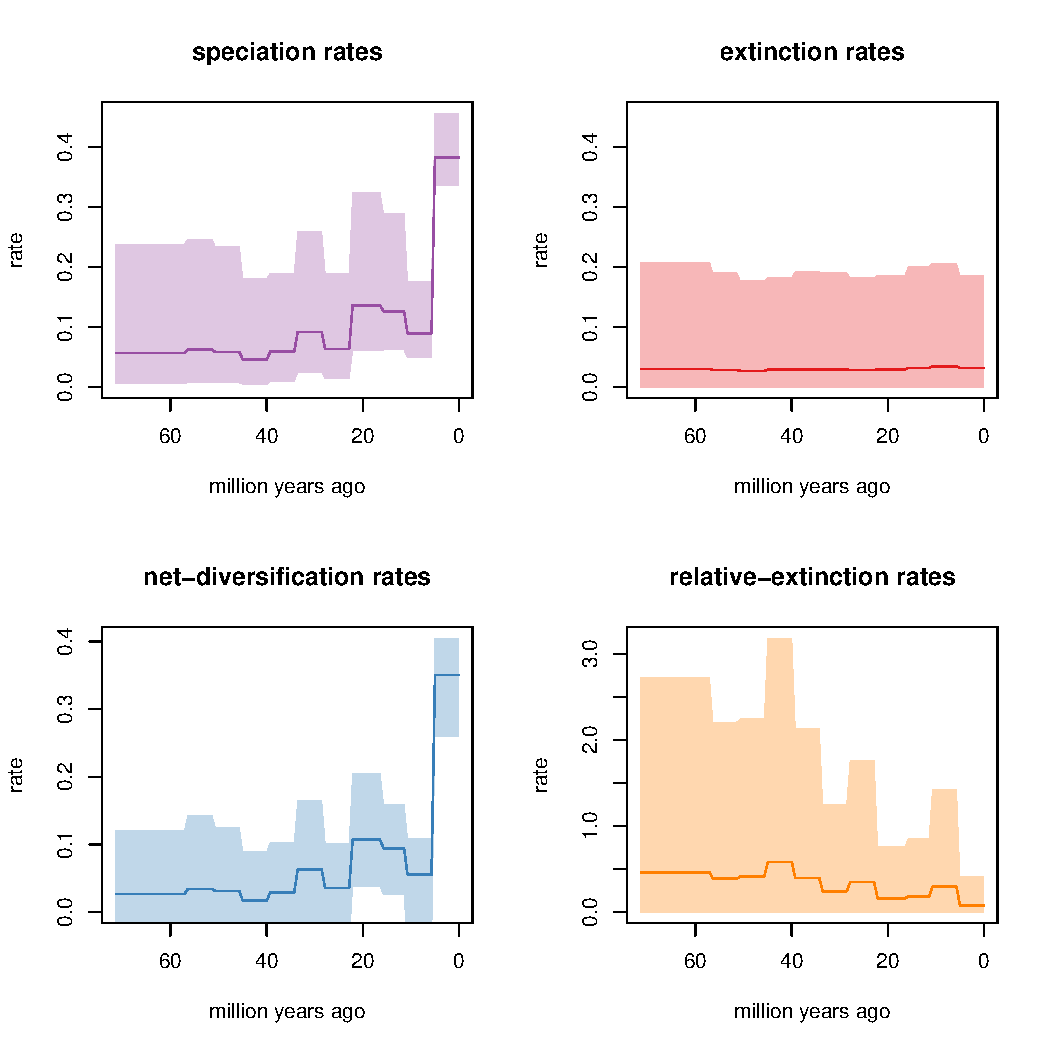
\includegraphics[width=\textwidth]{\ResourcePath figures/EBD_10_Result.pdf}}
\caption{\small Resulting diversification rate estimations when using 10 intervals. You should obtain similar results when you use 10 intervals. The estimated rates might change when you use a different resolution, \IE a different number of intervals.}
\label{fig:EBD_Results}
\end{figure}

\subsection{Exercise 1}

\begin{itemize}
\item Run an MCMC simulation to estimate the posterior distribution of the speciation rate and extinction rate.
\item Visualize the rate through time using \R.
\item Do you see evidence for rate decreases or increases? What is the general trend?
\item Is there evidence for rate variation? Look at the estimates of \cl{speciation\_sd} and \cl{extinction\_sd}: Is there information in the data to change the estimates from the prior?
\item Run the analysis using a different number of intervals, \EG 5 or 50. How do the rates change?
\end{itemize}


\subsection{Exercise 2}

\begin{itemize}
\item In our results we see that the extinction rate is fairly constant. Modify the model by using a constant-rate for the extinction rate parameter but still let the speciation rate vary through time.
\begin{itemize}
\item Remove all previous occurrences of the extinction rates (\IE priors, parameters and moves).
\item Specify a lognormal prior distribution on the constant extinction rate \\(\cl{extinction $\sim$ dnLognormal(-5,sd=2*0.587405)})
\item Add a move for the new extinction rate parameter \\\cl{moves[++mvi] = mvScale(extinction,weight=5.0)}.
\item Remove the argument \cl{muTimes=interval\_times} from the birth-death process.
\end{itemize}
\item How does this influence your estimated rates?
\end{itemize}



\bibliographystyle{sysbio}
\bibliography{\GlobalResourcePath refs}
